\documentclass[convert]{standalone}

\usepackage{tikz}
\usepackage{graphicx}
\pagestyle{empty}

% INT_AY22_L28-Fig07_Ampere_circuit_w_poly.png

\begin{document}
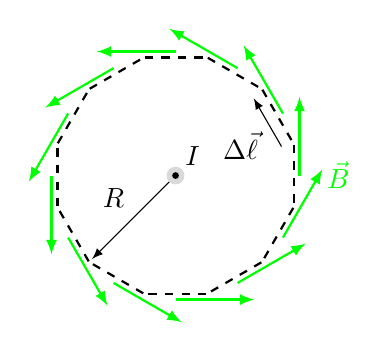
\begin{tikzpicture}[> = latex]

	% Definition
	
	\def\R{1.5}		% Size of amperian path
	\def\N{12} 		% Number of polygonal sides
	
	% Polygon segments + B vectors
	
	\foreach \Q in {0, 30, ..., 330}
	{
	
		% Polygon segments
		
		\coordinate (left) at ({\R * cos(\Q) - 3.14 * \R / \N * sin(\Q)}, {\R * sin(\Q) + 3.14 * \R / \N * cos(\Q)});
		\coordinate (right) at ({\R * cos(\Q) + 3.14 * \R / \N * sin(\Q)}, {\R * sin(\Q) - 3.14 * \R / \N * cos(\Q)});
		
		\draw [dashed, thick] (left) -- (right);
		
		% Field vectors
		
		\draw [thick, green, ->] (\Q : 1.05 * \R) -- ++ ({\Q + 90} : 1);
	}
	
	% Sample segment distance vector
	
	\draw [->] ({0.9 * \R * cos(30) + 3.14 * 0.9 * \R / \N * sin(30)}, {0.9 * \R * sin(30) - 3.14 * 0.9 * \R / \N * cos(30)}) --
			node [below left] {$\Delta {\vec \ell}$} ({0.9 * \R * cos(30) - 3.14 * 0.9 * \R / \N * sin(30)}, {0.9 * \R * sin(30) + 3.14 * 0.9 * \R / \N * cos(30)});
	
	% Radius indicator
	
	\draw [->] (0, 0) -- node [above left] {$R$} (225 : \R);

	% Wire w/ current
	
	\filldraw [gray!30] (0, 0) circle (3 pt) node [black, above right] {$I$};
	\filldraw (0, 0) circle (1 pt);
	
	% Magnetic field vectors on path
		
	\node [right, green] at (1.2 * \R, 0) {${\vec B}$};

\end{tikzpicture}
\end{document}